\documentclass[twoside]{book}

% Packages required by doxygen
\usepackage{fixltx2e}
\usepackage{calc}
\usepackage{doxygen}
\usepackage[export]{adjustbox} % also loads graphicx
\usepackage{graphicx}
\usepackage[utf8]{inputenc}
\usepackage{makeidx}
\usepackage{multicol}
\usepackage{multirow}
\PassOptionsToPackage{warn}{textcomp}
\usepackage{textcomp}
\usepackage[nointegrals]{wasysym}
\usepackage[table]{xcolor}

% Font selection
\usepackage[T1]{fontenc}
\usepackage[scaled=.90]{helvet}
\usepackage{courier}
\usepackage{amssymb}
\usepackage{sectsty}
\renewcommand{\familydefault}{\sfdefault}
\allsectionsfont{%
  \fontseries{bc}\selectfont%
  \color{darkgray}%
}
\renewcommand{\DoxyLabelFont}{%
  \fontseries{bc}\selectfont%
  \color{darkgray}%
}
\newcommand{\+}{\discretionary{\mbox{\scriptsize$\hookleftarrow$}}{}{}}

% Page & text layout
\usepackage{geometry}
\geometry{%
  a4paper,%
  top=2.5cm,%
  bottom=2.5cm,%
  left=2.5cm,%
  right=2.5cm%
}
\tolerance=750
\hfuzz=15pt
\hbadness=750
\setlength{\emergencystretch}{15pt}
\setlength{\parindent}{0cm}
\setlength{\parskip}{3ex plus 2ex minus 2ex}
\makeatletter
\renewcommand{\paragraph}{%
  \@startsection{paragraph}{4}{0ex}{-1.0ex}{1.0ex}{%
    \normalfont\normalsize\bfseries\SS@parafont%
  }%
}
\renewcommand{\subparagraph}{%
  \@startsection{subparagraph}{5}{0ex}{-1.0ex}{1.0ex}{%
    \normalfont\normalsize\bfseries\SS@subparafont%
  }%
}
\makeatother

% Headers & footers
\usepackage{fancyhdr}
\pagestyle{fancyplain}
\fancyhead[LE]{\fancyplain{}{\bfseries\thepage}}
\fancyhead[CE]{\fancyplain{}{}}
\fancyhead[RE]{\fancyplain{}{\bfseries\leftmark}}
\fancyhead[LO]{\fancyplain{}{\bfseries\rightmark}}
\fancyhead[CO]{\fancyplain{}{}}
\fancyhead[RO]{\fancyplain{}{\bfseries\thepage}}
\fancyfoot[LE]{\fancyplain{}{}}
\fancyfoot[CE]{\fancyplain{}{}}
\fancyfoot[RE]{\fancyplain{}{\bfseries\scriptsize Generated by Doxygen }}
\fancyfoot[LO]{\fancyplain{}{\bfseries\scriptsize Generated by Doxygen }}
\fancyfoot[CO]{\fancyplain{}{}}
\fancyfoot[RO]{\fancyplain{}{}}
\renewcommand{\footrulewidth}{0.4pt}
\renewcommand{\chaptermark}[1]{%
  \markboth{#1}{}%
}
\renewcommand{\sectionmark}[1]{%
  \markright{\thesection\ #1}%
}

% Indices & bibliography
\usepackage{natbib}
\usepackage[titles]{tocloft}
\setcounter{tocdepth}{3}
\setcounter{secnumdepth}{5}
\makeindex

% Hyperlinks (required, but should be loaded last)
\usepackage{ifpdf}
\ifpdf
  \usepackage[pdftex,pagebackref=true]{hyperref}
\else
  \usepackage[ps2pdf,pagebackref=true]{hyperref}
\fi
\hypersetup{%
  colorlinks=true,%
  linkcolor=blue,%
  citecolor=blue,%
  unicode%
}

% Custom commands
\newcommand{\clearemptydoublepage}{%
  \newpage{\pagestyle{empty}\cleardoublepage}%
}

\usepackage{caption}
\captionsetup{labelsep=space,justification=centering,font={bf},singlelinecheck=off,skip=4pt,position=top}

%===== C O N T E N T S =====

\begin{document}

% Titlepage & ToC
\hypersetup{pageanchor=false,
             bookmarksnumbered=true,
             pdfencoding=unicode
            }
\pagenumbering{alph}
\begin{titlepage}
\vspace*{7cm}
\begin{center}%
{\Large My Project }\\
\vspace*{1cm}
{\large Generated by Doxygen 1.8.12}\\
\end{center}
\end{titlepage}
\clearemptydoublepage
\pagenumbering{roman}
\tableofcontents
\clearemptydoublepage
\pagenumbering{arabic}
\hypersetup{pageanchor=true}

%--- Begin generated contents ---
\chapter{Hierarchical Index}
\section{Class Hierarchy}
This inheritance list is sorted roughly, but not completely, alphabetically\+:\begin{DoxyCompactList}
\item \contentsline{section}{crew}{\pageref{classcrew}}{}
\item Q\+Dialog\begin{DoxyCompactList}
\item \contentsline{section}{credit}{\pageref{classcredit}}{}
\item \contentsline{section}{edit}{\pageref{classedit}}{}
\item \contentsline{section}{Edit\+Aud}{\pageref{class_edit_aud}}{}
\end{DoxyCompactList}
\item Q\+Main\+Window\begin{DoxyCompactList}
\item \contentsline{section}{Login}{\pageref{class_login}}{}
\item \contentsline{section}{Login}{\pageref{class_login}}{}
\end{DoxyCompactList}
\item Q\+Widget\begin{DoxyCompactList}
\item \contentsline{section}{Data\+Base}{\pageref{class_data_base}}{}
\item \contentsline{section}{showtata}{\pageref{classshowtata}}{}
\end{DoxyCompactList}
\item \contentsline{section}{stage}{\pageref{classstage}}{}
\end{DoxyCompactList}

\chapter{Class Index}
\section{Class List}
Here are the classes, structs, unions and interfaces with brief descriptions\+:\begin{DoxyCompactList}
\item\contentsline{section}{\hyperlink{class_data_base}{Data\+Base} }{\pageref{class_data_base}}{}
\item\contentsline{section}{\hyperlink{class_login}{Login} }{\pageref{class_login}}{}
\item\contentsline{section}{\hyperlink{classshowtata}{showtata} }{\pageref{classshowtata}}{}
\item\contentsline{section}{\hyperlink{class_s_q_l_c_o_n}{S\+Q\+L\+C\+ON} }{\pageref{class_s_q_l_c_o_n}}{}
\item\contentsline{section}{\hyperlink{classsql_settings}{sql\+Settings} }{\pageref{classsql_settings}}{}
\end{DoxyCompactList}

\chapter{Class Documentation}
\hypertarget{classcredit}{}\section{credit Class Reference}
\label{classcredit}\index{credit@{credit}}
Inheritance diagram for credit\+:\begin{figure}[H]
\begin{center}
\leavevmode
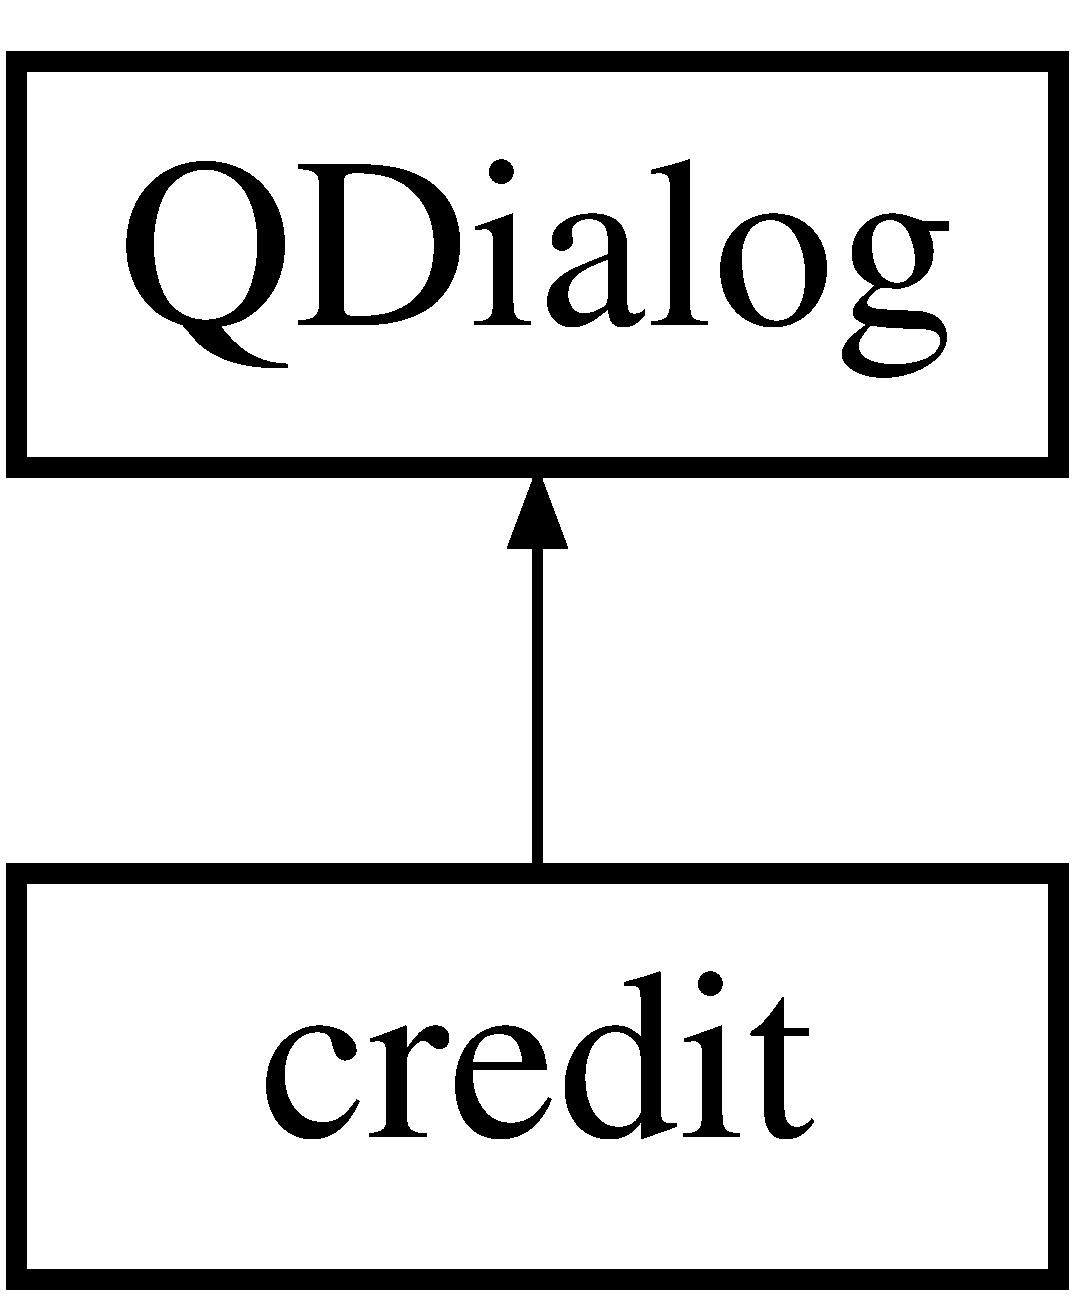
\includegraphics[height=2.000000cm]{classcredit}
\end{center}
\end{figure}
\subsection*{Public Member Functions}
\begin{DoxyCompactItemize}
\item 
\hypertarget{classcredit_a834ab6df70c91d8c4dde059f19d1fde7}{}\label{classcredit_a834ab6df70c91d8c4dde059f19d1fde7} 
{\bfseries credit} (Q\+Widget $\ast$parent=0)
\end{DoxyCompactItemize}


The documentation for this class was generated from the following files\+:\begin{DoxyCompactItemize}
\item 
credit.\+h\item 
credit.\+cpp\end{DoxyCompactItemize}

\hypertarget{classcrew}{}\section{crew Class Reference}
\label{classcrew}\index{crew@{crew}}
\subsection*{Public Member Functions}
\begin{DoxyCompactItemize}
\item 
\hypertarget{classcrew_a6e456cfd0ae54351c9b905697a16e7a8}{}\label{classcrew_a6e456cfd0ae54351c9b905697a16e7a8} 
{\bfseries crew} (Q\+String, Q\+String, Q\+String, float, int, int)
\item 
\hypertarget{classcrew_a4dc7e14c8f45f77de3fa71ab37a04704}{}\label{classcrew_a4dc7e14c8f45f77de3fa71ab37a04704} 
Q\+String {\bfseries get\+Car} () const
\item 
\hypertarget{classcrew_a9e026f669a61e2c4da28e5bdd5e11ce8}{}\label{classcrew_a9e026f669a61e2c4da28e5bdd5e11ce8} 
void {\bfseries set\+Car} (Q\+String)
\item 
\hypertarget{classcrew_af0075b1ca3dc6d7307030bc30cae025b}{}\label{classcrew_af0075b1ca3dc6d7307030bc30cae025b} 
Q\+String {\bfseries get\+Model} () const
\item 
\hypertarget{classcrew_a78b8e25ca2c3019c994c1f1e44fa1519}{}\label{classcrew_a78b8e25ca2c3019c994c1f1e44fa1519} 
void {\bfseries set\+Model} (Q\+String)
\item 
\hypertarget{classcrew_a7e095f7e2750a9caf3b92df2d6f8c420}{}\label{classcrew_a7e095f7e2750a9caf3b92df2d6f8c420} 
Q\+String {\bfseries get\+Drivetrain} () const
\item 
\hypertarget{classcrew_aaee38cf8aaf5091eb26c8d89b2fe1a4c}{}\label{classcrew_aaee38cf8aaf5091eb26c8d89b2fe1a4c} 
void {\bfseries set\+Drivetrain} (Q\+String)
\item 
\hypertarget{classcrew_a8633ef062b9eaec13a3ed11f8b02cd0f}{}\label{classcrew_a8633ef062b9eaec13a3ed11f8b02cd0f} 
float {\bfseries get\+Vol} () const
\item 
\hypertarget{classcrew_ac5403c12bfc2e3b9cb63c93681ecff49}{}\label{classcrew_ac5403c12bfc2e3b9cb63c93681ecff49} 
void {\bfseries set\+Vol} (float)
\item 
\hypertarget{classcrew_acc286896ae75c9f12942e87e228432d6}{}\label{classcrew_acc286896ae75c9f12942e87e228432d6} 
int {\bfseries get\+Power} () const
\item 
\hypertarget{classcrew_a4d85c4284a0cddbb742346e72e097640}{}\label{classcrew_a4d85c4284a0cddbb742346e72e097640} 
void {\bfseries set\+Power} (int)
\item 
\hypertarget{classcrew_a80f7b8bc3835dc92734217cf92157b82}{}\label{classcrew_a80f7b8bc3835dc92734217cf92157b82} 
int {\bfseries get\+Id} () const
\end{DoxyCompactItemize}


The documentation for this class was generated from the following files\+:\begin{DoxyCompactItemize}
\item 
crew.\+h\item 
crew.\+cpp\end{DoxyCompactItemize}

\hypertarget{class_data_base}{}\section{Data\+Base Class Reference}
\label{class_data_base}\index{Data\+Base@{Data\+Base}}
Inheritance diagram for Data\+Base\+:\begin{figure}[H]
\begin{center}
\leavevmode
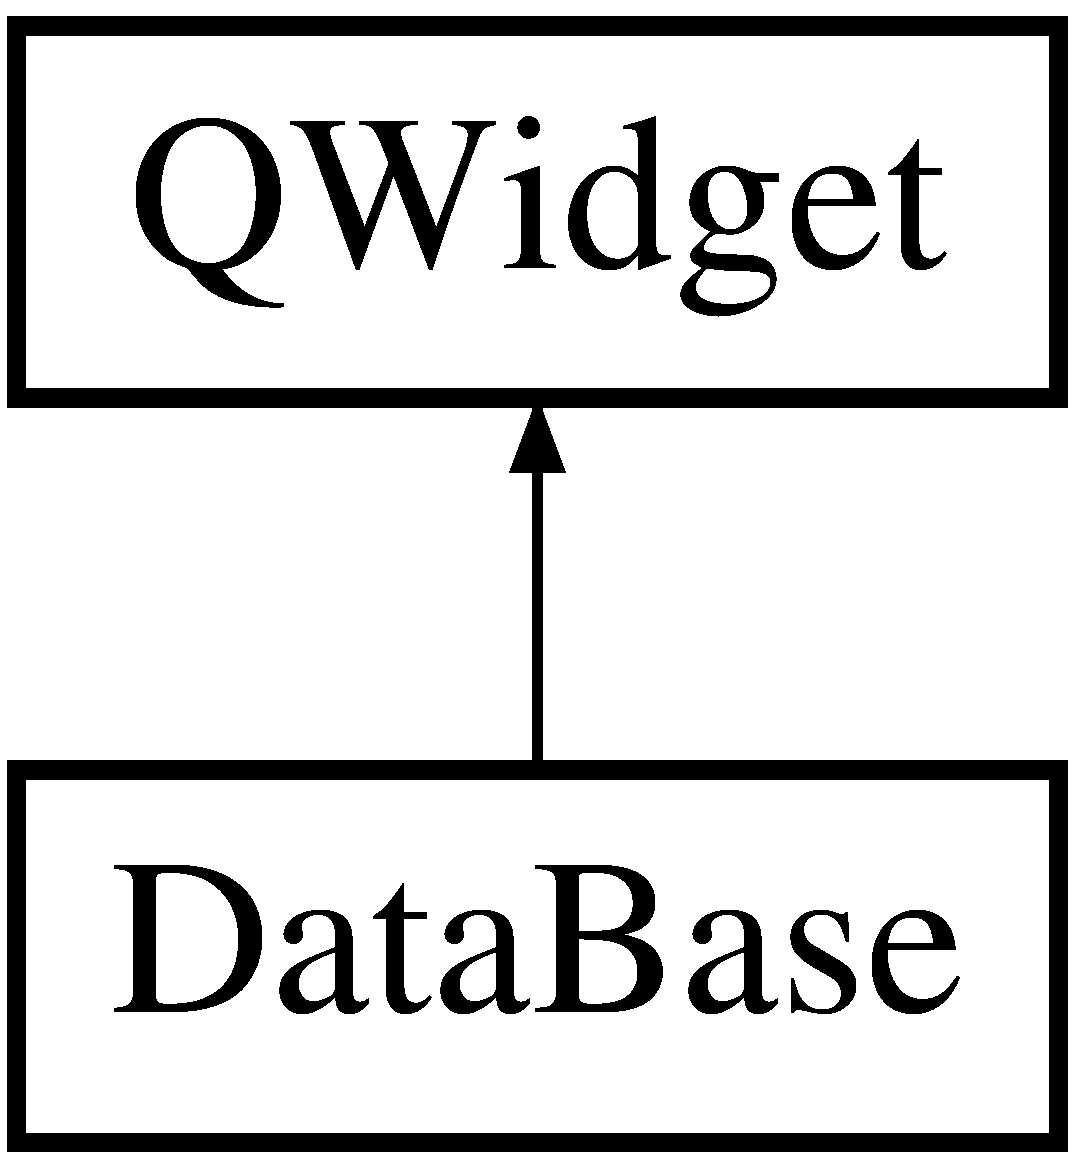
\includegraphics[height=2.000000cm]{class_data_base}
\end{center}
\end{figure}
\subsection*{Public Member Functions}
\begin{DoxyCompactItemize}
\item 
\hypertarget{class_data_base_a54fde8aa4dfdc9ce978f2985877caf6c}{}\label{class_data_base_a54fde8aa4dfdc9ce978f2985877caf6c} 
{\bfseries Data\+Base} (Q\+Widget $\ast$parent=0)
\end{DoxyCompactItemize}


The documentation for this class was generated from the following files\+:\begin{DoxyCompactItemize}
\item 
database.\+h\item 
database.\+cpp\end{DoxyCompactItemize}

\hypertarget{classedit}{}\section{edit Class Reference}
\label{classedit}\index{edit@{edit}}
Inheritance diagram for edit\+:\begin{figure}[H]
\begin{center}
\leavevmode
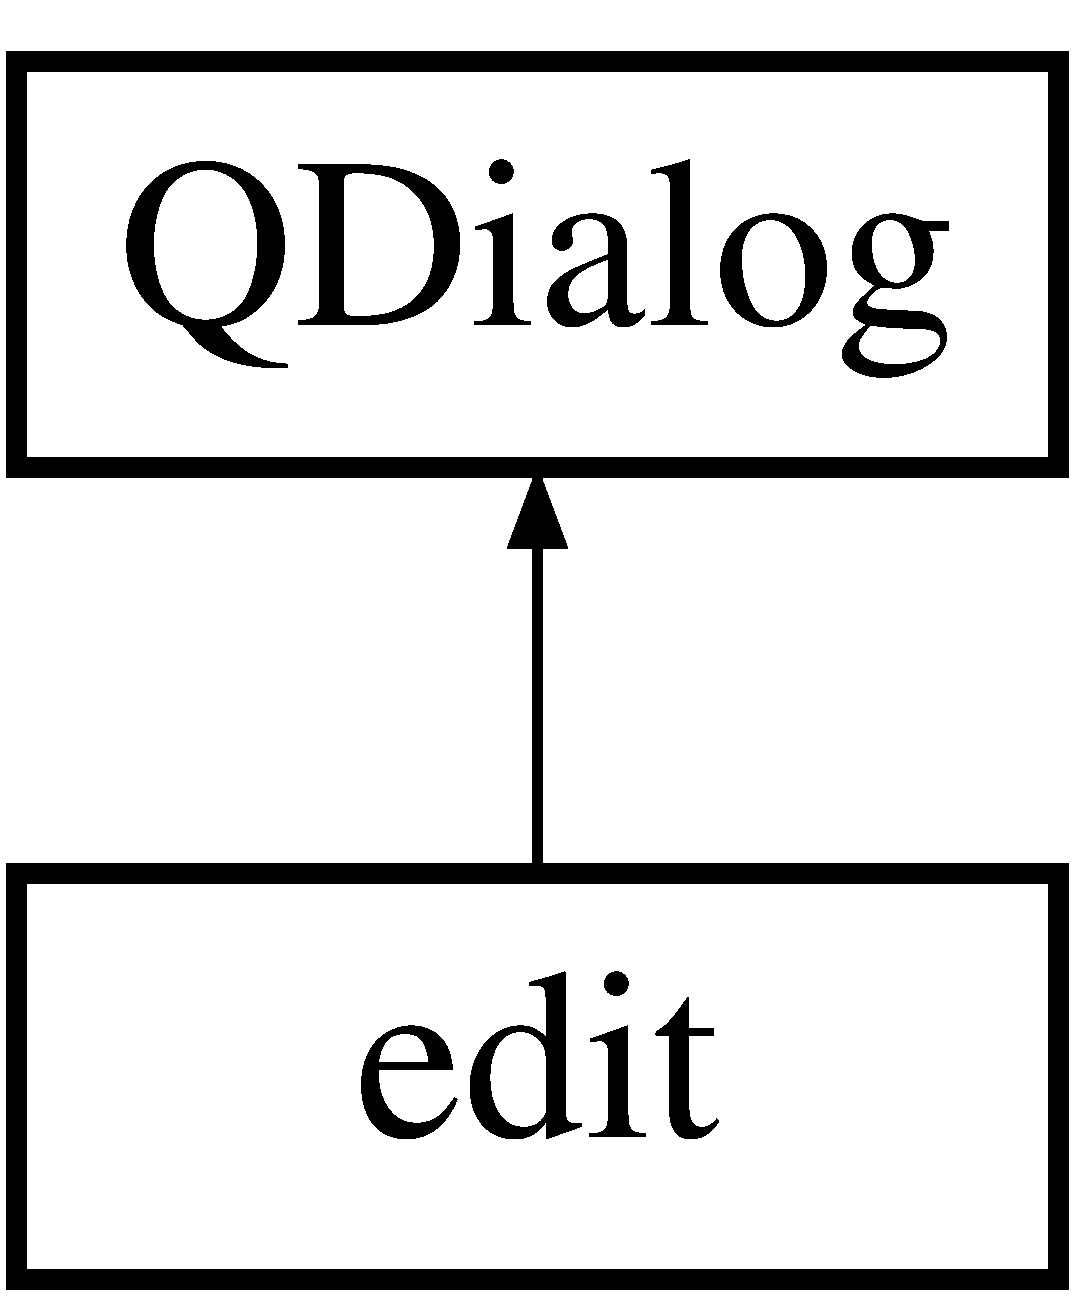
\includegraphics[height=2.000000cm]{classedit}
\end{center}
\end{figure}
\subsection*{Public Member Functions}
\begin{DoxyCompactItemize}
\item 
\hypertarget{classedit_a5eb3bc1268962c3352f3b3de164daeac}{}\label{classedit_a5eb3bc1268962c3352f3b3de164daeac} 
{\bfseries edit} (Q\+Widget $\ast$parent=0)
\item 
\hypertarget{classedit_adabb1ab89e251396613f548859401408}{}\label{classedit_adabb1ab89e251396613f548859401408} 
void {\bfseries addemployee} ()
\item 
\hypertarget{classedit_afeae840fba36b9ae5bab7937093666ae}{}\label{classedit_afeae840fba36b9ae5bab7937093666ae} 
void {\bfseries deleteemployee} ()
\item 
\hypertarget{classedit_a4d28ed1ecb81b8a9a0a3fbcd15503094}{}\label{classedit_a4d28ed1ecb81b8a9a0a3fbcd15503094} 
void {\bfseries setuptable} ()
\end{DoxyCompactItemize}


The documentation for this class was generated from the following files\+:\begin{DoxyCompactItemize}
\item 
edit.\+h\item 
edit.\+cpp\end{DoxyCompactItemize}

\hypertarget{class_edit_aud}{}\section{Edit\+Aud Class Reference}
\label{class_edit_aud}\index{Edit\+Aud@{Edit\+Aud}}
Inheritance diagram for Edit\+Aud\+:\begin{figure}[H]
\begin{center}
\leavevmode
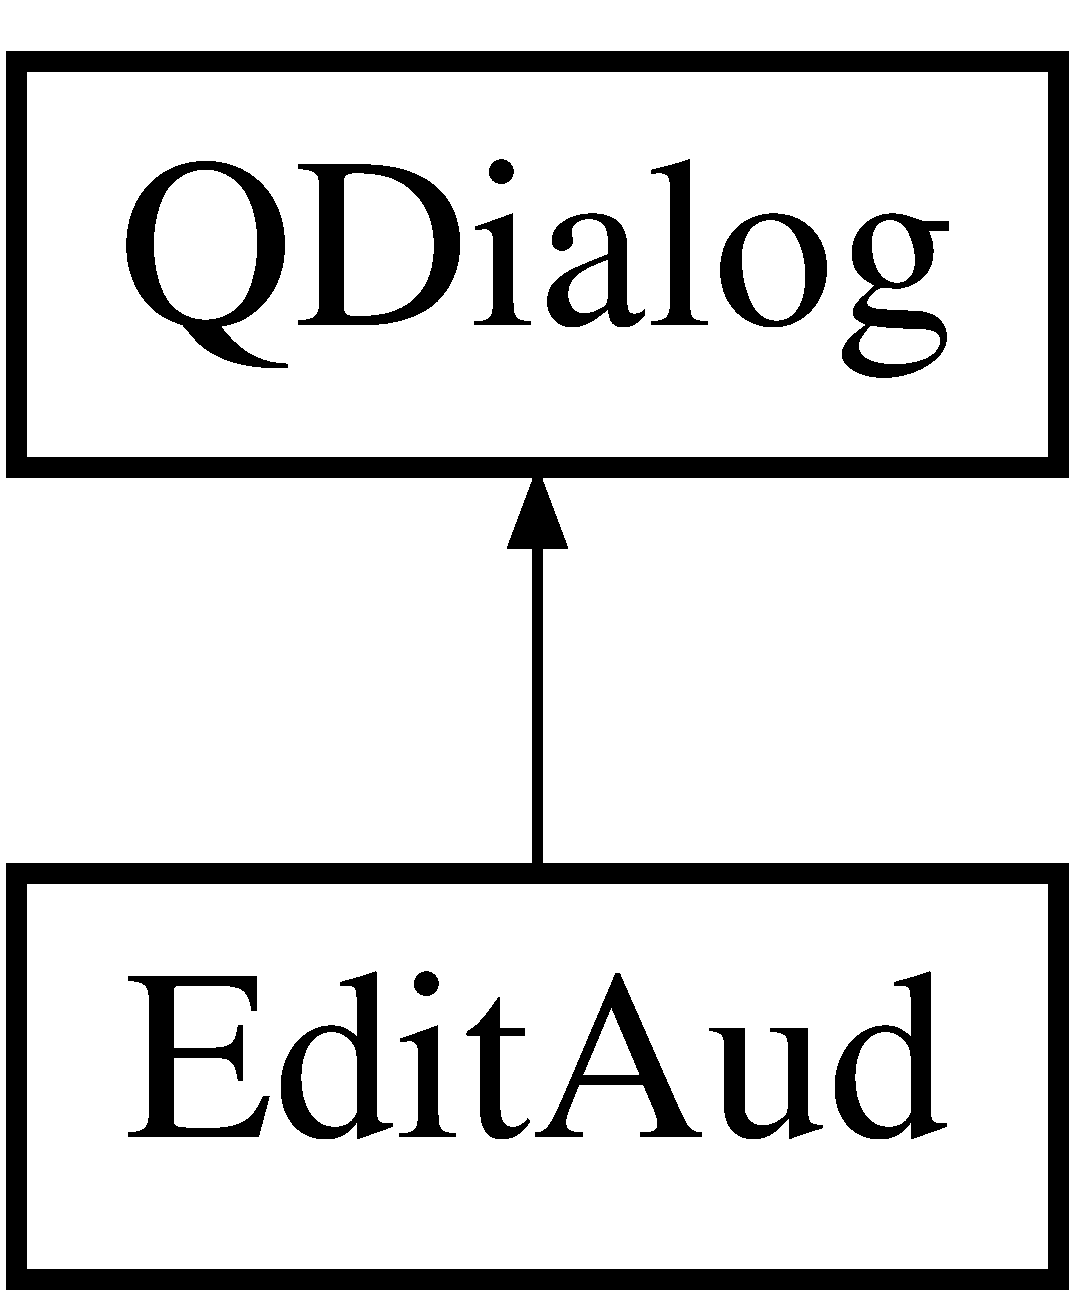
\includegraphics[height=2.000000cm]{class_edit_aud}
\end{center}
\end{figure}
\subsection*{Public Member Functions}
\begin{DoxyCompactItemize}
\item 
\hypertarget{class_edit_aud_a8aa69d8880550b5bde8d6f6c39ad5f39}{}\label{class_edit_aud_a8aa69d8880550b5bde8d6f6c39ad5f39} 
{\bfseries Edit\+Aud} (Q\+Widget $\ast$parent=0)
\item 
\hypertarget{class_edit_aud_adfe615e92f2227885bb93def076093bf}{}\label{class_edit_aud_adfe615e92f2227885bb93def076093bf} 
void {\bfseries addaud} ()
\item 
\hypertarget{class_edit_aud_a9562ccf126f504c7bfa12e4680673c20}{}\label{class_edit_aud_a9562ccf126f504c7bfa12e4680673c20} 
void {\bfseries deleteaud} ()
\item 
\hypertarget{class_edit_aud_a5e9c6752850192ac7c9e8574cc2d83b5}{}\label{class_edit_aud_a5e9c6752850192ac7c9e8574cc2d83b5} 
void {\bfseries editaud} ()
\item 
\hypertarget{class_edit_aud_a26608050cfa4ea590d06bca5b06dd040}{}\label{class_edit_aud_a26608050cfa4ea590d06bca5b06dd040} 
void {\bfseries setuptable} ()
\end{DoxyCompactItemize}


The documentation for this class was generated from the following files\+:\begin{DoxyCompactItemize}
\item 
editaud.\+h\item 
editaud.\+cpp\end{DoxyCompactItemize}

\hypertarget{class_login}{}\section{Login Class Reference}
\label{class_login}\index{Login@{Login}}
Inheritance diagram for Login\+:\begin{figure}[H]
\begin{center}
\leavevmode
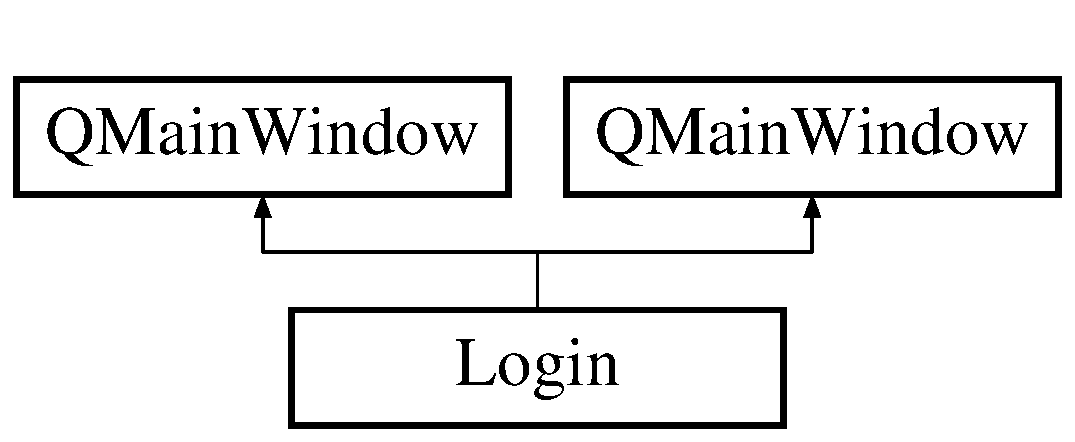
\includegraphics[height=2.000000cm]{class_login}
\end{center}
\end{figure}
\subsection*{Public Member Functions}
\begin{DoxyCompactItemize}
\item 
\hypertarget{class_login_a021ebcfd29b2a30e3f5c5bbb36589381}{}\label{class_login_a021ebcfd29b2a30e3f5c5bbb36589381} 
{\bfseries Login} (Q\+Widget $\ast$parent=0)
\item 
\hypertarget{class_login_ad6a6b037140e8823d1b290cbcfeb2087}{}\label{class_login_ad6a6b037140e8823d1b290cbcfeb2087} 
void {\bfseries loadsettings} ()
\item 
\hypertarget{class_login_aac2415f9743fe56e19c5488fabf4aaba}{}\label{class_login_aac2415f9743fe56e19c5488fabf4aaba} 
void {\bfseries savesettings} ()
\item 
\hypertarget{class_login_a5060f9bd0638df8820f80ecde59c801f}{}\label{class_login_a5060f9bd0638df8820f80ecde59c801f} 
void {\bfseries set\+Begin\+Seting} ()
\item 
\hypertarget{class_login_a021ebcfd29b2a30e3f5c5bbb36589381}{}\label{class_login_a021ebcfd29b2a30e3f5c5bbb36589381} 
{\bfseries Login} (Q\+Widget $\ast$parent=0)
\item 
\hypertarget{class_login_ad6a6b037140e8823d1b290cbcfeb2087}{}\label{class_login_ad6a6b037140e8823d1b290cbcfeb2087} 
void {\bfseries loadsettings} ()
\item 
\hypertarget{class_login_aac2415f9743fe56e19c5488fabf4aaba}{}\label{class_login_aac2415f9743fe56e19c5488fabf4aaba} 
void {\bfseries savesettings} ()
\item 
\hypertarget{class_login_a5060f9bd0638df8820f80ecde59c801f}{}\label{class_login_a5060f9bd0638df8820f80ecde59c801f} 
void {\bfseries set\+Begin\+Seting} ()
\end{DoxyCompactItemize}
\subsection*{Public Attributes}
\begin{DoxyCompactItemize}
\item 
\hypertarget{class_login_aeab33b7e36bd3e55c6a957290a74e221}{}\label{class_login_aeab33b7e36bd3e55c6a957290a74e221} 
Q\+Action $\ast$ {\bfseries Setting}
\item 
\hypertarget{class_login_a8c0727b99b15f38a77ab946fa3239801}{}\label{class_login_a8c0727b99b15f38a77ab946fa3239801} 
Q\+Message\+Box $\ast$ {\bfseries mes1}
\item 
\hypertarget{class_login_af88cd8be1e64096bdca27d016e60e719}{}\label{class_login_af88cd8be1e64096bdca27d016e60e719} 
\hyperlink{classshowtata}{showtata} $\ast$ {\bfseries dod}
\item 
\hypertarget{class_login_a7033035a95e1f9ab15f9ed9c2da9ceeb}{}\label{class_login_a7033035a95e1f9ab15f9ed9c2da9ceeb} 
\hyperlink{class_login}{Login} $\ast$ {\bfseries main}
\end{DoxyCompactItemize}


The documentation for this class was generated from the following files\+:\begin{DoxyCompactItemize}
\item 
login.\+h\item 
login\+\_\+copy.\+h\item 
login.\+cpp\end{DoxyCompactItemize}

\hypertarget{classshowtata}{}\section{showtata Class Reference}
\label{classshowtata}\index{showtata@{showtata}}
Inheritance diagram for showtata\+:\begin{figure}[H]
\begin{center}
\leavevmode
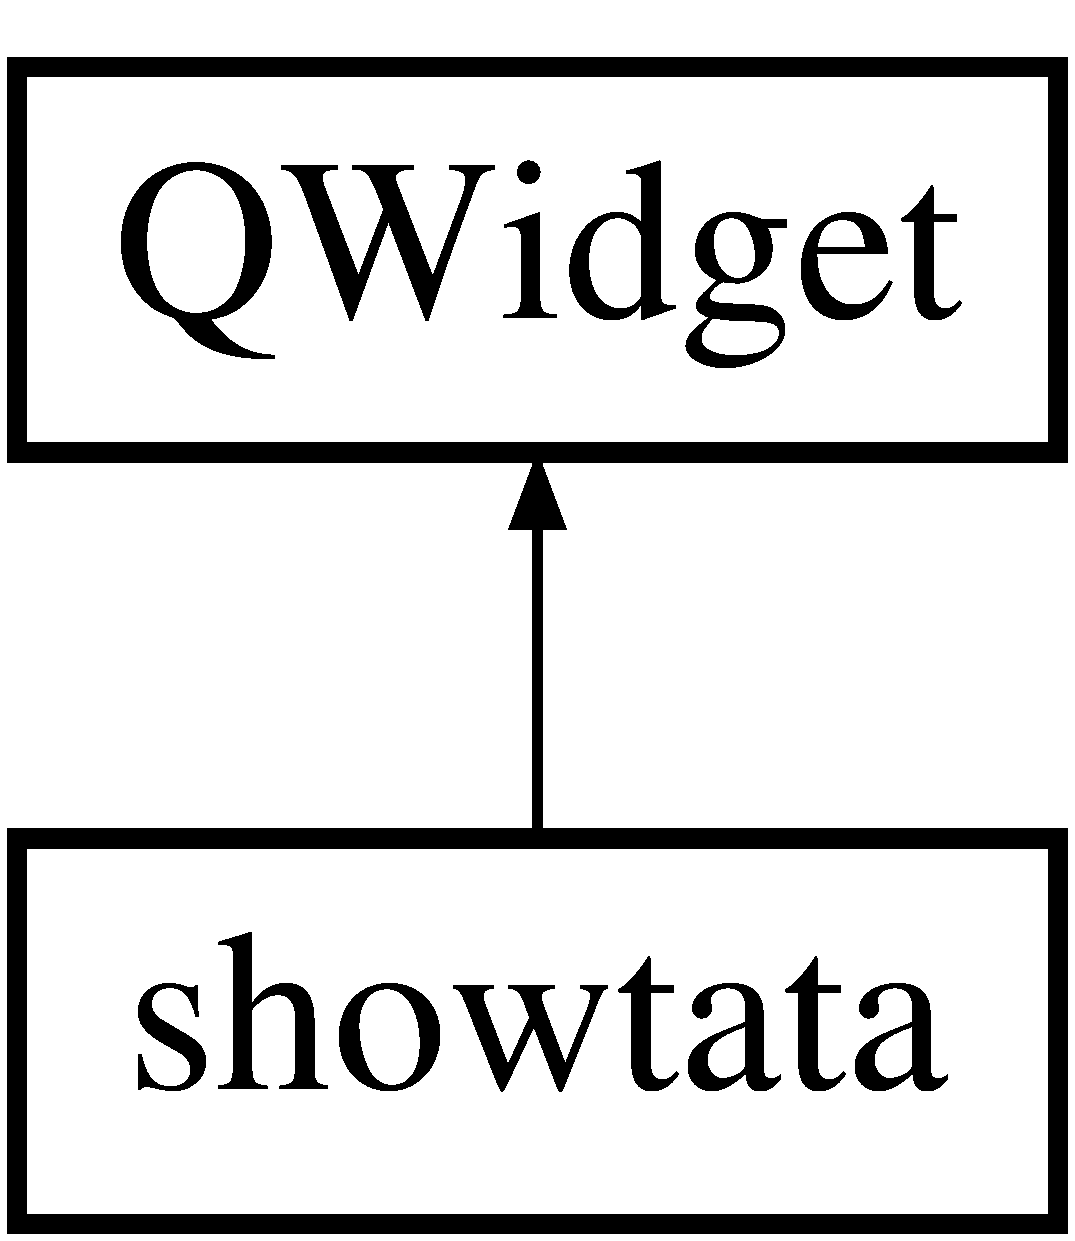
\includegraphics[height=2.000000cm]{classshowtata}
\end{center}
\end{figure}
\subsection*{Signals}
\begin{DoxyCompactItemize}
\item 
\hypertarget{classshowtata_af7c54c814de835f906e841b9ecaa6643}{}\label{classshowtata_af7c54c814de835f906e841b9ecaa6643} 
bool {\bfseries closed} ()
\end{DoxyCompactItemize}
\subsection*{Public Member Functions}
\begin{DoxyCompactItemize}
\item 
\hypertarget{classshowtata_a8b9382b64c639b083122cf4a5cee975d}{}\label{classshowtata_a8b9382b64c639b083122cf4a5cee975d} 
{\bfseries showtata} (Q\+Widget $\ast$parent=0)
\end{DoxyCompactItemize}
\subsection*{Public Attributes}
\begin{DoxyCompactItemize}
\item 
\hypertarget{classshowtata_a221cbd798a46ba1c75062e358bc17ad2}{}\label{classshowtata_a221cbd798a46ba1c75062e358bc17ad2} 
\hyperlink{classedit}{edit} $\ast$ {\bfseries edemp}
\item 
\hypertarget{classshowtata_ace79d422d191a7cf665c216495250a62}{}\label{classshowtata_ace79d422d191a7cf665c216495250a62} 
\hyperlink{class_edit_aud}{Edit\+Aud} $\ast$ {\bfseries edaud}
\end{DoxyCompactItemize}


The documentation for this class was generated from the following files\+:\begin{DoxyCompactItemize}
\item 
showtata.\+h\item 
showtata.\+cpp\end{DoxyCompactItemize}

\hypertarget{classstage}{}\section{stage Class Reference}
\label{classstage}\index{stage@{stage}}
\subsection*{Public Member Functions}
\begin{DoxyCompactItemize}
\item 
\hypertarget{classstage_ade7007cfb7d4668e970b91c7c113b622}{}\label{classstage_ade7007cfb7d4668e970b91c7c113b622} 
{\bfseries stage} (Q\+String, float, Q\+Time, int)
\item 
\hypertarget{classstage_abe5315b20cf10aa622a29fc2063f1135}{}\label{classstage_abe5315b20cf10aa622a29fc2063f1135} 
Q\+String {\bfseries get\+Name} () const
\item 
\hypertarget{classstage_a9317565c15e58922bc38b7254d00c9b3}{}\label{classstage_a9317565c15e58922bc38b7254d00c9b3} 
void {\bfseries set\+Name} (Q\+String)
\item 
\hypertarget{classstage_adde52511308b9e3b08faaaaa1c9d8607}{}\label{classstage_adde52511308b9e3b08faaaaa1c9d8607} 
float {\bfseries get\+Length} () const
\item 
\hypertarget{classstage_a0b298a3eb0be3eff6d26c4bd769597ad}{}\label{classstage_a0b298a3eb0be3eff6d26c4bd769597ad} 
void {\bfseries set\+Length} (float)
\item 
\hypertarget{classstage_a4eec9a2cd8216b276c6f7f9ee6b1b702}{}\label{classstage_a4eec9a2cd8216b276c6f7f9ee6b1b702} 
Q\+Time {\bfseries get\+Time} () const
\item 
\hypertarget{classstage_aae2add83f27cf81d5921c7e19409b84f}{}\label{classstage_aae2add83f27cf81d5921c7e19409b84f} 
void {\bfseries set\+Time} (Q\+Time)
\item 
\hypertarget{classstage_ad63f04d22f5873a42bd8b69c67be3fa1}{}\label{classstage_ad63f04d22f5873a42bd8b69c67be3fa1} 
int {\bfseries get\+Id} () const
\end{DoxyCompactItemize}


The documentation for this class was generated from the following files\+:\begin{DoxyCompactItemize}
\item 
stage.\+h\item 
stage.\+cpp\end{DoxyCompactItemize}

%--- End generated contents ---

% Index
\backmatter
\newpage
\phantomsection
\clearemptydoublepage
\addcontentsline{toc}{chapter}{Index}
\printindex

\end{document}
